\documentclass{report}
\usepackage[utf8]{inputenc}
\usepackage[danish]{babel}
\usepackage{amsmath}
\usepackage{graphicx}
\usepackage{subfig}
\usepackage{appendix}
\begin{document}

%Forside
\title{Projektarbejde, Snake}
\date{18. januar, 2015}
\author{	Anna Ølgaard Nielsen - 			s144437\\
Christian Søholm Andersen 	- s103080\\
Mathias Enggrob Boon - 			s144484\\
Van Anh Tri Trinh - 				s144449}

\maketitle
%Indholdfortegnelse
\pagenumbering{gobble}
\tableofcontents
\newpage
%Første side
\setcounter{chapter}{0}
\pagenumbering{arabic}
\chapter{Introduktion}
Formålet med projektopgaven er at genskabe det klassiske spil \textbf{Snake}, samt at dokumentere hvordan spillet er lavet.
Spillet er gengivet i to versioner: \textbf{Simpel Snake} og \textbf{Avanceret Snake}. 

Simpel Snake er en primitiv version af spillet, hvor styring og bevægelse kun foregår vha. input fra spilleren (se figur \ref{fig:simplesnake}). 

I Avanceret Snake er der tilføjet forskellige funktioner, som enten forbedrer brugerfladen - f.eks. tilføjelse af hovedmenu - eller ændrer spillets funktioner - f.eks. automatisk bevægelse af slangen (se figur \ref{fig:advancedsnake}).

I rapporten vil designet af begge spillets versioner blive forklaret, samt implementationen af spillet. Kapitlet \textit{Udviklingsproces} forklarer de tanker, der ligger bag implementationen, og de valg der er foretaget, i situationer med flere forskellige muligheder.

\begin{figure}[b]
	\centering
	\graphicspath{ {pics/} }
	\subfloat[Simpel Snake]{\label{fig:simplesnake}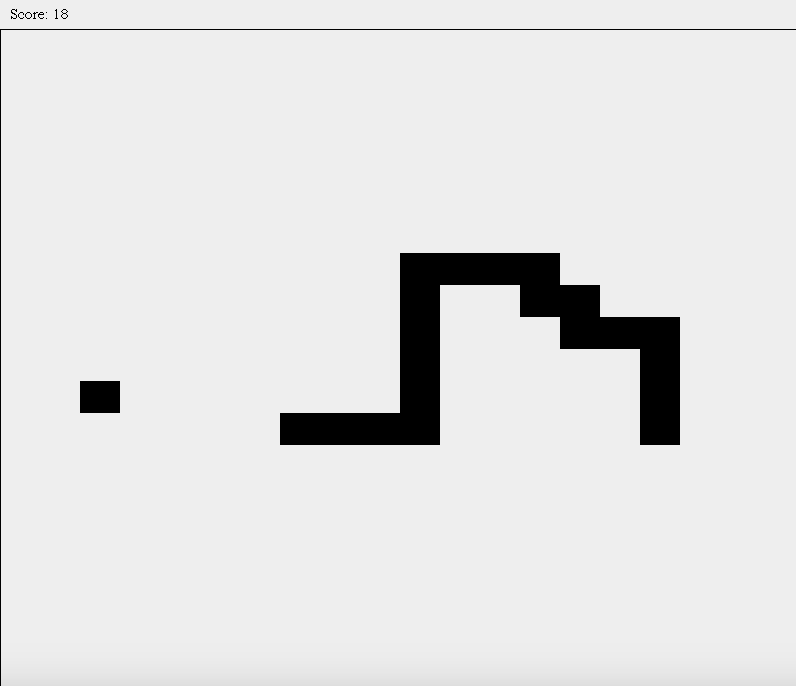
\includegraphics[width=0.4\textwidth]{SimpelSnake.png}}
	\hspace{0.1\textwidth}
	\subfloat[Advanced Snake]{\label{fig:advancedsnake}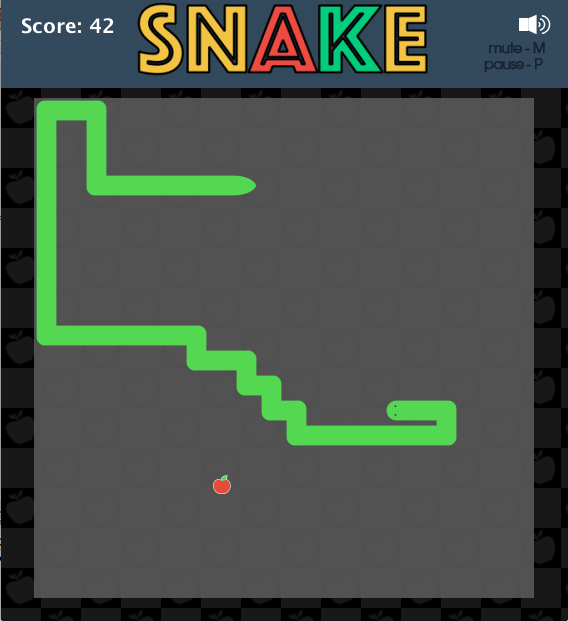
\includegraphics[width=0.32\textwidth]{snake2.png}}
	\caption{}
\end{figure}

\chapter{Simpel Snake}
\section{Afgrænsning}
I Simpel Snake består slangen af to felter (et hoved og en hale), der er placeret i banens centrum med hovedet rettet mod venstre. Det er muligt gennem input fra tastaturet at bevæge sig frit på banen i de fire retninger i et almindeligt koordinatsytem: op og ned ad y-aksen og hen ad x-aksen i begge retninger - dog ikke modsatrettet slangens bevægelsesretning. Bevæger man sig ud over banens kanter, fortsætter slangen på den modsatte side. Det skal derudover være muligt at øge slangens længde ved at bevæge sig over et felt med et æble. Spillet slutter, når spilleren har fyldt hele banen ud med slangens krop og dermed har vundet spillet, eller ved at spilleren bevæger sig ind i et felt udfyldt af slangen, der ikke er halestykket, da halestykket ved slangens bevægelse også rykker videre til et nyt felt. I så fald, har spilleren tabt.

\section{Design}
Snake-spillet er lavet efter et \textit{Model-View-Controller}-design (MVC), hvorved selve spillet, styringen af spillet og den visuelle repræsentation af spillet holdes adskilt i tre dele. På denne måde interagerer brugeren kun med den del af programmet, der er dedikeret til styring. Styringen manipulerer programmets tilstand i \textit{model}-koden, som visualiseres i \textit{view}-koden. Dette betyder derfor også, at alle funktioner, der påvirker programmets tilstand, skal holdes i \textit{model}-koden. \textit{Control} modtager kun input fra brugeren, og sender dette videre til \textit{View} og/eller \textit{Model}. \textit{View} modtager input fra \textit{Control} og sender ændringerne i \textit{View} videre til \textit{Model}. Det er derefter muligt gennem en observer at "observere" ændringerne i \textit{Game}, som bliver opdateret i \textit{View}.

Simpel Snake er designet, så spillets funktioner ligger i klassen \textit{Game} i model-pakken. \textit{Game} får da spillets objekter fra andre klasser i \textit{model}-pakken, f.eks. Level (banen) og Snake (slangen). Spillets tilstand ændres, når der modtages input fra control-klasserne, som bestemmer hvornår og hvordan slangen bevæger sig. I \textit{BoardPanel}-klassen er en observer, som notificeres hver gang banens tilstand ændres. Når dette sker, eller når spillet startes, tegnes banen vha. klasserne \textit{View} og \textit{BoardPanel}. Disse klasser modtager information fra model-klasserne, f.eks. \textit{Snake}, til at bestemme hvordan spillet tegnes. \textit{BoardPanel} gentegner hele spillet hver gang spillet opdateres. Først tegnes selve banen, derefter slangen og til sidst æblet. 

For at starte spillet bruges klassen \textit{Driver}, som opretter et nyt \textit{Game}-, \textit{View} og \textit{Control}-objekt.



\section{Implementering}
\subsection{Control (Styring)}
I Simpel Snake bruges kun fire taster til input, nemlig de fire piletaster, som derfor er defineret i \textit{Control}.\textit{Control}-klassen har metoden \textit{keyPressed}, som kommer af at \textit{Control}-klassen implementerer \textit{KeyListener}, som kaldes hver gang der tastes på tastaturet. Hvis tasten er en af de fire piletaster, kaldes funktionen \textit{move} i \textit{Snake}-klassen, der flytter hovedet i samme retning som piletasten.
Enum-klassen \textit{Direction} indholder \textit{RIGHT, LEFT, UP} og \textit{DOWN}. Dette bruges i \textit{Control}-klassen, da det ikke skal være muligt at bevæge sig i modsatte retning af slangens nuværende retning.
I \textit{Control}-klassens constructor er Direction som udgangspunkt sat til \textit{LEFT}, da slangen starter mod venstre. Hver gang der tastes på piletasterne, sikrer \textit{keyPressed}-metoden, at retningen ikke er modsat af den nuværende retning. Herefter flyttes slangen, uanset om den er midt på spillepladen eller om den bevæger sig rundt om torussen. Til sidst sættes \textit{Direction} til den nuværende retning, så det ved næste tasteanslag igen kan undersøges, at retningen ikke er modsat.

\subsection{Model}
Spillets model består af en række klasser, der tilsammen udgør selve spillets funktioner og objekter.
Klassen \textit{Field} bruges til at definere et et punkt, som repræsenterer et felt i banen. Den fungerer på samme måde som \textit{Point}-objekt-klassen, hvor koordinatsystemet starter oppe i venstre hjørne. Forskellen mellem \textit{Point}- og \textit{Field}-klassen, er hvordan man kommer frem til et punkt. \textit{Point}-klassen går først ud ad x-aksen og derefter ned ad y-aksen, hvorimod \textit{Field}-klassen gør det i omvendt rækkefølge. Da hele spillepladen er delt op i rækker og kolonner, frem for en x- og y-akse, er \textit{Field} lettere at bruge for at undgå forvirring, dato-dimensionelle arrays også er opdel i rækker og kolonner, hvor den første værdi repræsenterer rækker, mens den anden værdi repræsenterer kolonner..

Funktionenen \textit{equals} er defineret i denne klasse, og bruges til at undersøge om to objekter ligger på samme felt, f.eks. slangens hoved og æblet. Æblet bliver oprettet i klassen \textit{Game}, hvor datafeltet \textit{position} afgør dets nuværende position.

Slangen selv er defineret i klassen \textit{Snake}. Slangens krop består af en række felter, hvoraf det første er hovedet, og de resterende er kroppen inklusiv halen til sidst. Koordinaterne for disse felter er gemt som elementer i en ArrayList kaldet \textit{positions}. Det første element er slangens første led, hovedet, det andet element er slangens andet led osv. Når et nyt led tilføjes, tilføjes et nyt element til listen. Dette sker, når slangen spiser et æble, hvor den ikke bevæger sig som ellers. I stedet tilføjes et nyt hoved på æblets felt. Hovedets retning er den samme, som slangens sidste bevægelse.

I \textit{Snake}-constructoren bliver slangens hoved og hale oprettet, hvor hovedet bliver placeret i banens centrum. Halen placeres i kolonnen til højre for på samme række.

I \textit{move}-metoden benyttes Action-klassen, der er oprettet som en enum, og betegner slangens handlinger: om slangen spiser et æble, er død eller bevæger sig (hhv. \textit{EAT, KILL, MOVE}). I \textit{move}-metoden undersøges der, om der er mad på samme felt som hovedets nye placering. Er dette tilfældet, bliver Action-statementet til \textit{EAT}. Hvis ikke, undersøges der om den nye placering for hovedet allerede indeholder slangens krop. Gør der det, bliver Action-statementet til \textit{KILL}. Hvis ikke, flyttes slangens hoved til den nye position. Resten af slangens krop følger med ved at ændre koordinaterne i \textit{positions} fra halen og op til hovedet, dvs. at halens koordinater bliver næstsidste led, næstsidste bliver tredjesidste osv. Slangens krop flyttes først, hvorefter hovedet flyttes til sidst, for at undgå at andet led indtager samme plads som hovedet.

I \textit{Game}-klassen findes \textit{checkAction}-metoden, der undersøger om slangen spiser eller dør. Hvis Action-statementet er \textit{EAT}, øges slangens længde ved at tilføje et nyt element på æblets felt, som fungere som nyt hoved. Scoren inkrementeres, der laves et nyt æble, og Action-statementet sættes til \textit{MOVE}.
Hvis Action-statementet er \textit{KILL}, nulstilles scoren, og spillet slutter ved at slangen ikke længere kan bevæge sig.
Herudover findes \textit{generateFood}-metoden, som sikrer, at maden altid placeres på et gyldigt felt, dvs. et felt der ikke er udfyldt af slangen. For at sikre dette, placeres æblet på et tilfældigt felt inden for banens rammer, hvorefter der undersøges om et af slangens led har samme koordinater som æblets felt. Er dette tilfældet, gives æblet et nyt felt, indtil det lander på et felt uden slangen. Er slangen tilpas stor, er dette dog ikke effektivt, da der er stor sandsynlighed for at ramme et felt, der er optaget af slangen. Af denne årsag undersøger metoden først, om slangen fylder mere end halvdelen af banen. Er dette tilfældet, laves der i stedet en liste med alle tomme felter vha. en indlejret for-løkke, der løber gennem alle række og kolonner, hvorefter et tilfældigt element i listen vælges som æblets position.

De fire klasser \textit{Food, Score, Game} og \textit{Snake} forlænger klassen \textit{Observable}, så det er muligt for View at modtage ændringerne i \textit{Model}, uden at \textit{Model} afhænger af View.

\subsection{View (Brugergrænseflade)}
Brugerfladen er samlet i klassen \textit{GameView} der forlænger \textit{JFrame}. I \textit{GameView} findes kun en constructor, hvor der oprettes et \textit{ScorePanel}-objekt, der placeres øverst i vinduet, og et \textit{BoardPanel} objekt, der placeres direkte under det. Board-panelet viser selve banen med slangen og æblet, der begge er vist ved farvede firkanter. 

\textit{ScorePanel}-klassen forlænger \textit{JPanel} og implementerer \textit{Observer}. Klassen har en \textit{update}-metode, der gentegner, hver gang noget ændrer sig i de klasser i model-pakken, der forlænger \textit{Observable}. 
\textit{paintComponent}-metoden benyttes til at tegne score-teksten. Selve panelet oprettes i constructoren.

\textit{BoardPanel} forlænger også \textit{JPanel} og implementerer \textit{Observer}, for at den også kan registerere ændringer i model-klasserne. \textit{BoardPanel} består af en række draw-metoder, samt en \textit{paintComponent}-metode, der kalder på draw-metoderne for at tegne alle spillets komponenter på spillets bane og spillets bane selv.
I \textit{drawSnake}-metoden bruges positionerne for slangens felter til at tegne slangen. Størrelsen for et felt udregnes i \textit{getWindowRectangle}-metoden, og afhænger af vinduets og banens størrelse. Når feltets størrelse er udregnet, tegnes en rektangel med feltets størrelse på alle felterne i slangens positions-ArrayList.

\section{Udviklingsproces}
\subsection{Arbejdsproces}
Formålet med projektet var at starte med at lave en simpel udgave af snake, og derefter tilføje flere funktioner for at lave en mere avanceret version. Dette gør det ideelt at tilføje én funktion ad gangen, frem for at planlægge alle funktioner på en gang, og tilføje dem samtidig. Resultatet bliver et, til at starte med, simpelt men fungerende program, hvorefter yderligere funktioner kan tilføjes. Programmet er altså udviklet iterativt, hvorved der opstår flere fungerende versioner af spillet, men med forskellige funktioner. Dette gør det muligt at tilpasse programmet, hvis der opstår nye idéer eller krav undervejs. 

Den iterative tilgang gør det muligt at have en "cyklus" for udviklingen af programmet. Først bestemmes det, der skal tilføjes til programmet. Derefter fordeles opgaverne blandt gruppens medlemmer. Gruppemedlemmet afgør selv, hvordan en funktion skal designes og implementeres, men sikrer at implementationen er kompatibel med alle nuværende funktioner, og ikke vil hindre fremtidige tilføjelser i at blive tilføjet. Eventuelle justeringer til programmet laves for at undgå fejl med nye funktioner, hvorefter "cyklussen" starter forfra ved idéfasen.

\subsection{Control}
Idet der ikke er brug for nogen menu eller lignende i Simpel Snake, er det muligt at holde styringen af spillet meget simpel. Ved at definere de fire piletaster i \textit{Control}-klassen, samt en funktion til at sikre at der ikke bevæges i modsat retning, er alle styringkrav til Simpel Snake opfyldt. Resten af spillet håndteres da i model-koden.

\subsection{Model}
\subsubsection{Opbygning af banen}
Til designet af banen, som slangen bevæger sig på, foreslås to muligheder. Den ene er at lave et to-dimensionelt array af datatypen enum, hvis størrelse afgør banens endelige størrelse. Et array [10][5] vil f.eks. give en bane med længden 10 og bredden 5. Hvert element i arrayet bestemmer da, hvad der befiner sig på netop denne plads på banen. Elementerne i arrayet kan f.eks. være et blankt felt, et æble, et led af slangen osv. Dette gør det nemt at introducere nye spilelementer i fremtiden, f.eks. bonus-point, vægge og miner, idet der blot skal tilføjes nye værdityper. Visualisering af spillet foregår ved at definere et billede for hvert spilelement, og få programmet til at tegne objektet på arrayets plads.

En anden metode er, at lade de forskellige spilelementer være defineret i deres egne klasser, så f.eks. \textit{SnakeFood} er en klasse for sig selv, \textit{SnakePlayer} er en klasse for sig selv osv. Hver klasse har de funktioner, der er relevante for dem, f.eks. \textit{getPosition} for at give deres nuværende position. Programmet tegner da spillet hver gang en tur afsluttes, dvs. når alle elementer som skal ændres, er ændret. Programmet har fået defineret billedet for de forskellige elementer, og modtager deres position vha. en \textit{getPosition} metode.
Ulempen ved denne metode er, at det skal laves flere metode og klasser, hvormed programmets kompleksitet stiger. I den første metode er alle felter allerede defineret, og for at ændre dem behøves værdien for hvert felt blot at blive ændret, så f.eks. et blankt felt ændres til æble. Ønskes et spilelement ændret eller introduceret med den anden metode, skal der laves et nyt objekt. Ønsker man at introducere nye elementer, kan man med første metode blot tilføje en ny værdi-type til det todimensionelle array. Med anden metode skal der laves nye klasser, metoder osv. for at introducere nye elementer til spillet.
 
I sidste ende blev metode 2 valgt, idet den gjorde det nemmere at holde Model-koden adskilt fra View- og Control-koden. Herudover har første metode den ulempe, at den skal sende et todimensionelt array på banens størrelse, hver gang banen skal tegnes. Ved en bane på f.eks. 100x100 betyder dette, at at sendes i alt 10000 elementer til View-koden, hver gang banen skal tegnes. Den anden metode sender derimod kun de relevante elementer, dvs. æblets og slangens position, til View-koden.

\subsubsection{Snake}
Da slangen i snake-spillet består af en række felter, som alle har netop en koordinat i forbindelse med andre led, er en effektiv måde at bestemme slangens position på en ArrayList, idet denne datastrukturer er fleksibel i størrelse og passer til formålet. Når slangen vokser i størrelse, bliver dette dog mindre effektivt, idet slangens hoved altid sættes som element 0. Når slangen vokser, tilføjes et nyt element på plads 0, hvormed hele listen skal flyttes. En anden mulighed ville være at bruge en anden datastruktur, f.eks. LinkedList, eller lade hovedet være defineret som element positions.size()-1, hvormed nye hovedet tilføjes sidst i listen. Et problem ved at bruge LinkedList er dog, at denne datastruktur ikke tillader vilkårlig adgang af værdier, men derimod altid bevæger sig fra første eller sidste element. Dette problem kan løses ved at bruge en iterator, men blev fravalgt, idet det skabte problemer, når listen skulle bruges på tværs af klasserne.

Til implementationen af scoren blev to løsninger foreslået. Enten at lade scoren være et datafelt i game-klassen, eller at lade det være en klasse for sig selv. Ved at lade scoren være et datafelt, bliver implementationen simplere. At lade scoren være en klasse for sig selv har derimod fordelen, at der kan 
tilføjes en observer til Score-klassen, som dermed kun opdateres, når scoren ændrer sig. Scorepanelet tegnes ikke i samme klasse som banen, og kan derfor holdes seperat, så scorepanelet kun gentegnes, når scoren ændrer sig. Hvis scoren derimod er et datafelt, tegnes scoren efter hver tur, også selvom scoren er uændret. I sidste ende blev det bestemt at holde scoren som datafelt, hvormed fremtidige score-relaterede funktioner bliver simplere at implementere.

\subsection{Brugerflade og visualisering af programmet}
\subsubsection{Tegning af spillet}
For at visualisere spillet er det nødvendigt at kunne optegne banen, slangen og æblet. Dette gøres i klassen ViewBoard, som har metoderne drawBackground, drawBoard, drawSnake og drawFood, som hver især tegner deres tilsvarende element. Metoden paintComponent kalder de førnævnte metoder, således at baggrunden tegnes først, så banen, så æblet og sidst slangen. Alting gentegnes hver gang spillet opdateres, hvormed der "tegnes over" det gamle billede. Det kan her argumenteres for, at f.eks. baggrunden ikke bør gentegnes, når slangen bevæger sig, lige som store dele af banen forebliver uændret, og derfor ikke behøver gentegnes. Alternativt kunne man lave et system, som undersøger hvilke områder der skal gentegnes, og hvilke der er uændret, og derfor ikke skal gentegnes. Dette kan dog i sidste ende betyde, at de kræfter der spares på tegning i stedet blot bruges på at afgøre, hvad der skal tegnes.

\subsubsection{Vinduesstørrelse}
Området, som spillet foregår på, skal kunne bestemmes til at være mellem 5x5 og 100x100. Dette kan dog skabe problemer, hvis størrelsen bliver for stor, idet banen både skal være synlig, men også passe på en gennemsnitlig computerskærm. En bane på 10x10 kan sagtens passe på en opløsning af f.eks. 400x400, men øges banens størrelse til 50x50, bliver banen svær at se. Herudover varierer skærmstørrelser, og det er derfor nødvendigt at gøre spillets vinduestørrelse fleksibel. En løsning på dette problem ville være at bestemme en fast størrelse for felterne, og lade vinduet justere sin størrelse efter dette. Ønskes det f.eks. at felterne altid har størrelsen 20x20, og at banen skal være 15x25, vil vinduets størrelse blive 300x500. Fordelen ved denne metode er at det sikres, at banen altid er synlig, og at der ikke opstår problemer, fordi forholdet mellem vinduets størrelse og banen størrelse ikke passer sammen. Ulempen ved metoden er, at store baner kan blive for store til at være på en normal skærm. F.eks. vil en bane med felter af størrelsen 20x20 og banestørrelsen 75x75 fylde 1500x1500. Herudover er løsningen ikke brugervenlig, idet en bruger kan blive forvirret over hvorfor vinduets størrelse ændrer sig fra bane til bane, og måske ligefrem ikke passer på skærmen.

En anden metode er at gøre vinduet justerbart. Denne løsning er mere brugervenlig, idet vinduets størrelse frit kan justeres så det passer til den enkelte person. Denne metode introducerer dog et andet problem, nemlig at felternes størrelse skal skaleres til at passe vinduet. Nogle opløsninger af vinduet vil ikke være et multiplum af banens størrelse, hvormed elementerne i spillet vil blive aflange. Dette problem bliver løst i avanceret snake ved at lave en baggrund og låse banens forhold, hvormed banen altid fylder mest muligt af vinduet ud, mens den beholder sin form, og den resterende plads bliver udfyldt af baggrunden. Idet denne løsning var nemmere at bruge og forstå, og giver bedre mulighed for justering af spillet, blev den valgt frem for den første løsning.
\begin{figure}[h]
	\centering
	\graphicspath{ {pics/} }
	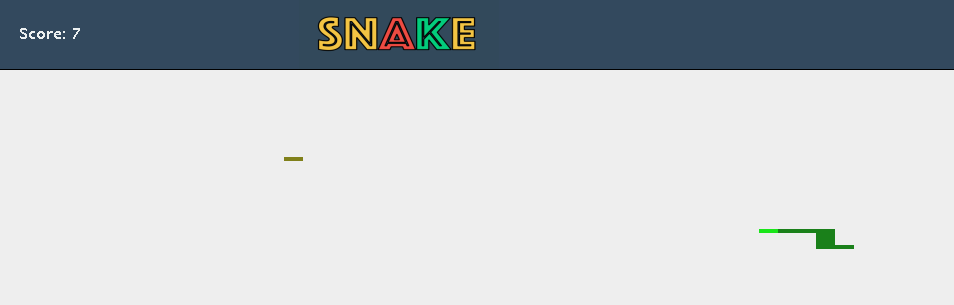
\includegraphics[width=0.5\textwidth]{WindowSize.png}
	\label{fig:windowsize}
	\caption{windowsize}
\end{figure}


\section{Evaluering}
-To eller en Arraylist -> linklist ?
-Point -> Field
-Int -> Enum (direction)
-width+height <-> kvadratisk variabel ?
-Banens opbygning: double-array -> positions-placering
-Optimering af runtime i “food”-klassen (dobbelt for-loop eller random placering)
-brug af observer - får model-view-controller til at gå op
-Flere opgaver er givet til “game”-klassen frem for de andre klasser

\chapter{Avanceret Snake}
I dette afsnit er den endelige version af Snake beskrevet. De dele af spillet, som også er brugt i Simpel Snake, og som ikke er blevet ændret, f.eks. justering af vinduesstørrelse, vil ikke blive forklaret i dette afsnit. //////

\section{Afgrænsning}
I den avancerede del af spillet bevæger slangen sig automatisk ved hjælp af en timer, og venter derfor ikke på input fra tastaturet. Input fra tastaturet bruges derimod til at skifte retning eller til at fremskynde den automatiske bevægelse. Derudover accelereres slangens hastighed, dvs. at tiden mellem hver automatisk bevægelse formindskes, efterhånden som spillerens score stiger, hvilket øger spillets sværhedsgrad. Der tilføjes også lydeffekter og dertil en mute-funktion. 
Vi har valgt at fokusere på et rent og fleksibelt design, der gør det let for spilleren at forstå og bevæge sig rundt mellem spillets scener. Derfor skal det være muligt både at kunne navigere igennem input fra tastaturet og musen. Udover spil-scenen tilføjes der en hovedmenu, der giver spilleren overblik over alle spillets scener, en hjælpe-scene, der forklarer hvordan man navigerer rundt i spillet og indstillingsscener, der indstiller spillet før det starter. Brugergrænsefladen skal også tilpasses brugerens ønskede vinduesstørelse og brugerens operativsystem. Før spillets start skal det i indstillingsscenen være muligt at vælge mellem forskellige starthastigheder, slangens farve og banens størrelse.
Med en multiplayer-implementation, bliver det også muligt at kunne spille to spillere på samme bane, hvor spilleren ikke længere alene skal undgå at bide sig selv, men også undgå at støde ind i sin modspiller.

\section{Design}
I \textit{Driver}-klassen, hvori main-metoden for programmet ligger, oprettes to objekter fra de to hovedklasser \textit{View} og \textit{Control}, der hver især står for henholdsvis \textit{View} og \textit{Control} i \textit{Model-View-Controller}-designet. Klassen \textit{Game}, der står for \textit{Model}-delen oprettes først i hovedmenuens control-klasse \textit{ControlMenu}, da denne derved får lettere adgang til spillet, når spilleren trykker på menuens knapper. 

I JFrame'n \textit{View} er spillets forskellige komponenter opdelt i hver deres klasse. Disse view-klasser er alle JPanels som tilføjes til vinduet og skiftes ud alt efter spillets tilstand. Er spilleren f.eks. i hovedmenuen, bruges \textit{ViewMenu}-klassen til at tegne denne. Er spilleren i et multiplayer-spil, bruges \textit{ViewBoardMultiplayer} og \textit{ViewHeaderMultiplayer}. På denne måde har hver scene i spillet en tilhørende klasse der forlænger et JPanel. De fleste af view-klasserne oprettes alle med \textit{View} som parameter, og kan derfor give og bruge hinandens funktioner, idet \textit{View}-klassen har getter-metoder til de view-klasser, som oprettes i \textit{View}. View-klasserne kan derfor genbruge nødvendige metoder, f.eks. metoden til at tegne baggrunden op, som er defineret i \textit{ViewMenu}-.klassen. Spilleren navigerer vha. JButtons eller tastatur-input der modtages i control-klasserne.
View-klasserne består af \textit{Colors}, \textit{Images}, \textit{ViewAudio}, \textit{ViewBoard}, \textit{ViewBoardMultiplayer}, \textit{ViewBoardSingleplayer}, \textit{ViewControls}, \textit{ViewHeader}, \textit{ViewHeaderSingleplayer}, \textit{ViewHeaderMultiplayer}, \textit{ViewMenu}, \textit{ViewOptions}, \textit{ViewOptionsSingleplayer} og \textit{ViewOptionsMultiplayer}. [SE KLASSEDIAGRAM FOR RELATIONER....]
Al grafik, som ikke er fra \textit{Swing}-biblioteket, er importeret i klassen \textit{Images}, der gør det muligt for enhver view-klasse at få fat i alle billeder. På samme måde er selv-definerede farver oprettet i klassen \textit{Colors}.

\textit{Control}-klassen er konstrueret med \textit{View} som parameter, og virker derfor alle steder i spillet. \textit{Control}-klassen har funktioner som \textit{mute} og \textit{return to menu}, som skal være fungerende uanset hvor i spillet spilleren er, og dermed uanset hvilke paneler der er vist. I samme pakke ligger andre control-klasser, som alle hører til en bestemt scene. Dette sikrer, at der kun bliver givet de styringfunktioner, som er nødvendige i den nuværende scene.

I \textit{Model}-pakken findes den abstrakte klasse \textit{Game}, som klasserne \textit{GameSingleplayer} og \textit{GameMultiplayer} implementerer. Klasserne har handlinger (MOVE, EAT, LOSE, WIN, START, PAUSE, RESUME) og spiltilstande (isStarted, isRunning, isPaused, isEnded) tilfælles, men har forskellige mål, der derfor er defineret i hver deres klasse, mens de fælles funktioner ligger i superklassen.

\section{Implementering}
\subsection{Model}
Modellen er nu lavet så det er muligt at vælge mere end én spiller. I både \textit{GameSingleplayer} og \textit{GameMultiplayer} findes en timer hvor det dog kun er i Singleplayer-spillet at timerens opdateringsinterval formindskes efter hvert femte samlet æble. Slangen er stadig defineret som en ArrayList i klassen \textit{Snake}, hvor også dens [.......................]

\subsubsection{Multiplayer}

\subsection{View (Brugergrænseflade)}
Ændret siden simpel: Tilføjede scener. Brug af importerede billeder. Optegning af slange efter bevægelse.


Når \textit{View}-klassen konstrueres, opretter den i sin constructor \textit{ViewAudio}-, \textit{ViewMenu}-, \textit{ViewHeader}- og \textit{ViewControls}-objekter. \textit{ViewAudio}-klassen står for spillets lyde, der spilles efter slangens handlinger i spilscenen hvis klassens Boolean felt \textit{muted} er falsk. \textit{ViewHeader} er en topbar, som indeholder spillets titel, tastatur-genveje og en JButton, der viser om lyden er slået til eller fra og som ligeledes kan bruges til at slå lyden til eller fra. \textit{ViewMenu}-panelet indeholder JButtons som giver spilleren adang til spillets scener: Singleplayer, Multiplayer og Controls - der fører til hjælpescenen \textit{ViewControls}. Desuden har den også en \textit{Quit}-knap, som fungerer som vinduets kryds i hjørnet. Når \textit{View} oprettes i \textit{Driver}-klassen og sættes til visible, kører den først \textit{showMenu}-metoden, der tilføjer \textit{ViewHeader}-panelet og \textit{ViewMenu}-panelet. Disse skiftes kun ud med andre paneler gennem input fra spilleren, når spilleren bevæger sig rundt i spillet. Dette sker med \textit{View}s \textit{setFrameComponents} metode, der tager to komponenter som parametre, hvorefter Frame'n skifter dens nuværende indhold ud med de to nye paneler. Frame'n bruger \textit{BorderLayout}, der gør det simpelt at placere et header-panel øverst, og det ønskede scene-panel nedenunder. Alle andre view-klasser er efterladt med standard-layoutet \textit{FlowLayout}, da deres komponenter skal placeres i specifikke koordinater. Dette gøres med \textit{setLocation} der definerer komponentets præcise placering ved x- og y-koordinater. Når spilleren ændrer vinduets størrelse, er deres koordinater dog ikke altid bevaret hvis komponenterne f.eks. altid skal ligge i midten af vinduet. Disse kald på \textit{setLocation}-metoden er derfor placeret i panelernes \textit{paintComponent}-metode da, denne køres hver gang vinduet skaleres. Koordinaterne beregnes derved påny hver gang vinduet skaleres, og komponenterne kan derfor altid få de rigtige koordinater. Denne metode er brugt til alle billeder, JComponents og tekst der oprettes eller tegnes.

((((((((((Klikkes der på \textit{Singleplayer}- eller \textit{Multiplayer}-knappen, skiftes menu-panelet ud med henholdsvis \textit{ViewOptioinsSinglePlayer} eller \textit{ViewOptionsMultiplayer}, der hver viser indstillings-scenerne for hver game-mode. Klasserne har superklassen \textit{ViewOptions}, der tegner baggrunden, skriver tekst, opretter input-felter til valg af bane, konsturerer sværhedsgradsknapper og play- og back-knapper. Underklasserne opretter selv deres farve-knapper, da der for multiplayer skal være otte knapper i alt, mens singleplayer kun har fire forskellige knapper. Gå man videre herfra vha. play-knappen, skiftes panelerne endnu engang ud med enten \textit{ViewHeaderSingleplayer} og \textit{ViewBoardSinglePlayer} eller \textit{ViewHeaderMultiplayer} og \textit{ViewBoardSingleplayer} der er underklasser til \textit{ViewHeader} og \textit{ViewBoard}.)))))) - Design?


(((((((I klassen \textit{ViewBoard} tegnes grafikken til spillet. Her er lagt specielt vægt på, at felternes størrelse passer til spillerens ønskede bane-størrelse og spillerens ønskede vinduesstørrelse samtidig med at bevare deres kvadrate form. Metoden \textit{getFieldSideLength} beregner ud fra disse to størrelser den størst mulige længde og højde af et enkelt felt og returnerer derefter den mindste af de to værdier. På denne måde kan feltet være kvadratisk og passer med sikkerhed på begge led af vinduet. Denne \textit{getFieldSideLength}-metode kan nu bruges til at bestemme størrelsen af og tegne banen, slangen og æblet, så de passer til vinduets størrelse. Da disse tegnemetoder bliver kaldt fra \textit{paintComponent}-metoden, der køres igennem konstant under spillet og når vinduesstørelsen ændres, har spillets komponenter altid en passende størrelse.))))))))))- gentaget?
Når spilleren færdiggør spillet enten ved at tabe eller vinde, tegnes \textit{Game Over}-skærmen ved en gennemsigtig rektangel, med \textit{Final Score} og JButtons, der giver mulighed for at gå tilbage til menuen eller spille igen.
Udover bane-størrelse er det også muligt at vælge slangens farve. Når en farve er valgt tjekkes der i \textit{drawSnake}-metoden i \textit{ViewBoard}-klassen om farven har været valgt før. Hvis ikke tilføjes den nye farve til ArrayListen \textit{snakeColors}, mens alle billederne som udgør slangen farves og bruges til at tegne slangen. Hvis farven har været valgt før, behøves billederne ikke at farves igen, men kan hentes i hvert billedes egen ArrayListe. Billederne farves ved at køre hver enkel pixel igennem ved en indlejret for-løkke og derefter give det en anden farve defineret ved tre heltal givet som parametre til \textit{colorSnakeImage}-metoden, der farver den givne pixel, hvis dens farve ikke er svarende til slangens øjenfarve.

\subsection{Control (Styring)}
Ændret siden simpel: Mute, pause, escape, enter.

For at give spilleren valgfrihed er der til mange funktioner både implementeret en JButton og en tilhørende genvej gennem tastaturet. Fra tastaturet er der blevet implementeret følgende genveje: Mute-knap (M), pause-knap (P), menu-knap (Esc), tilbage-knap (Backspace) og (re)start-knap (enter/space). \textit{Control}-klasserne [extends] \textit{KeyAdapter}, der registerer tastatur-input, og implementerer \textit{ActionListener}, der registrerer tryk på JButtons. Disse klasser tilføjer \textit{KeyListeners} til \textit{View}-klassen, og \textit{ActionListener} til hver enkel knap, der har funktioner i ActionListenerens tilhørende klasse. Individuel kontrol over de forskellige knapper fås ved at sætte en unik \textit{ActionCommand} til hver enkel knap, der derefter kan tjekkes for i ActionListeneren abstrakte metode \textit{actionPerformed}. Det er her også nødvendigt efter knappetryk at bruge \textit{requestFocus}-metoden på \textit{View}-klassen, da spillet efter knappetryk, får et nyt fokus, hvilket betyder, at tastatur-inputtet ikke opfattes af spillet.
Især når \textit{View} oprettes, bruges \textit{setFocusable}- og \textit{requestFocus}-metoderne, eftersom tastatur-input allerede skal være brugbart når spillet åbnes på grund af \textit{mute}-funktionen.

\textit{Control}-klassen er en global klasse, der står for kontrollen overalt i spillet. Dvs. muligheden for at slå lyden til eller fra eller vende tilbage til menuen. Når enten (M) eller lydknappen trykkes på, sættes \textit{ViewAudio}-klassens boolean 'mute' til det modsatte af det den i forvejen var, mens \textit{ViewHeader} (eller dens underklasser) notificeres for at opdatere lyd-ikonet. [INSERT PIC]
\textit{ControlBoardMultiplayer} og \textit{ControlBoardSingleplayer} indeholder metoden \textit{actionPerformed}, der genstarter eller går ud af spillet når spilleren trykker på 'Play Again'-knappen eller 'Menu'-knappen. Klasserne indeholder også KeyEvents, som kalder på en \textit{move}-metode i \textit{GameSingleplayer} eller \textit{GameMultiplayer}, der får slangen til at bevæge sig, når spilleren trykker på tastatur-tasterne, som styrer slangen. Klasserne indeholder også KeyEvents'ene (P), der fryser spillet og (ENTER)/(SPACE), der fungerer som 'Play Again' knappen.

\textit{ControlOptions}, der er en abstrakt klasse implementeret af \textit{ControlOptionsSingleplayer} og \textit{ControlOptionsMultiplayer}, styrer knapperne i indstillings-scenerne. Før spillets start kan spilleren som tidligere nævnt - udover at vælge farve og sværhedsgrad - vælge banestørrelsen. Denne funktion er indbygget vha. to \textit{JFormattedTextFields} der har fået en \textit{Formatter}, som begrænser inputtet til højst et tre-cifret tal. Dette begrænser spillerens mulighed for at indtaste en ugyldig størrelse. Trykkes på en af farve-knapperne eller sværhedsgrads-knapperne, optegnes den vha. JButton-metoden \textit{setBorder} med en tyk kant, for at vise at den er aktiv, mens kanterne på de andre knapper fjernes med \textit{setBorderPainted(false)}. Trykkes på en farveknap, sendes farven til \textit{ViewBoard}s \textit{setSnakeColor}-metode, der derefter bruger farven som beskrevet tidligere. Trykkes på en sværhedsgradsknap, sættes  en 'Difficulty' enum til den valgte sværhedsgrad. Denne bruges når 'Play'-knappen trykkes eller der trykkes (ENTER). 'Play'-knappen kalder på den implementerede abstrakte metode \textit{playAgain}, som først tjekker om tekst-felterne for bane-størrelsen er tomme, da der så printes en fejlmelding. For ikke at gøre det for svært for spilleren at indtaste en gyldig værdi, ses der bort fra eventuelle mellemrum før, i eller efter tallene. Dette gøres med metoden \textit{getInput} i superklassen, der fjerner alle mellemrum. Der undersøges derefter om tallene ligger mellem 5 og 100. Hvis dette er tilfældet, sættes bane-størrelsen vha. game-klassernes \textit{setBoardSize}-metodem, sværhedsgraden sættes med \textit{setSpeed}-metoden, spillet nulstilles (i tilfælde af at det har været startet før) og startes.

(((((((Da tekstfelterenes \textit{Formatter} får deres caret til at sætte sig i starten af tekstfeltet selvom spilleren trykker et andet sted i feltet, implementerer \textit{ViewOptions}-klassen en \textit{FocusListener}, der har de abstrakte metoder \textit{focusGained} og \textit{focusLost(...)}. I \textit{focusGained} oprettes )))))).

\section{Udviklingsproces}
\subsection{Control}
Diskussion: Opdeling af controlklasser

\subsection{Model}
\subsubsection{Menu}
Forklaring af

\subsubsection{Multiplayer}
Singleplayer og multiplayer

\subsubsection{Automatisk bevægelse}
Timer og acceleration


\subsection{View}
\subsubsection{Tegning af slangen}
Ændret siden simpel: Undersøgelse af slangens led

I Simpel Snake kan spilleren ud fra slangens krop se hvor han har været, men ikke hvilken vej han har bevæget sig, idet de udfyldte felter er fyldt helt ud til kanten[FIG HENVISNING]. Slangens udseende kan derfor forbedres ved at vise slangens bevægelsesretning og retningsskift i hver enkel del af dens krop og generelt erstatte alle firkanterne, med mere beskrivende billeder [FIG HENVISNING]. Dette giver seks mulige udseender for hver enkel del af slangen udover hovedet og enden af halen, der hver findes i fire versioner afhængig af retningen, som spilleren vælger for hovedet, eller retningen af kropsdelen lige før halen. Kropsstykkerne imellem er dog ikke kun afhængig af retningen af stykket lige før eller lige efter, men begge dele. Den vandrette del og den lodrette del af slangen bestemmes let ved at undersøge om stykket, der skal tegnes ligger i samme række eller kolonne som stykkerne før og efter. Slangens hjørnestykker bestemmes på en mere indviklet måde, da stykket og dens tilgrænsende stykker aldrig ligger i samme række eller kolonne, men derimod kan ligge i fire forskellige forhold til hinanden (Se figur 3.1). I figur \ref{fig:corner1} ligger de tilgrænsende felter lige under og til højre for hjørnet, men dette gælder f.eks. ikke for figur \ref{fig:corner3} hvor det ene stykke ligger lige under, mens det andet stykke ligger til venstre for hjørnet uden at grænse op til dens venstre side, der ellers ville give hjørnestykket spejlvendt i y-aksen. Da felterne ligger i en XXXXX-liste sorteret efter slangens opnåede dele, sammenlignes et felt med feltet før og efter det i listen. Da stykket foran og bagved uden påvirkning på hjørnestykket kan bytte plads, findes der altså otte situationer for et enkelt hjørnestykke. I alt tjekkes der derfor - for kroppen alene - 34 mulige forhold mellem et stykke og dens to tilgrænsende stykker.
\linebreak

I \textit{ViewBoard}-klassen er der lavet en \textit{drawSnake}-metode, der består af en del if-statements, for hvilket figur af slangen, der skal bruges i en bestemt retning. I \textit{snakeCorner}-metoden returnerer den en lang boolean \textit{isCorner}, som tidligere har været kopieret 4 gange for de fire retninger, men som nu er blevet simplificeret med en masse variable til den samme boolean. Måden det blev gjort på, var at finde et mønster i de fire lange booleans før og så indsætte 12 forskellige varibale, der gjorde det muligt kun at kalde en boolean. På samme tid kører programmet ikke alle if-else-statements igennem hver gang den skal lave et hjørne, men kun det hjørne som bliver kaldt. Variablerne kan enten have værdien 0, 1, -1, lastColumn eller lastRow. Da det specifikke hjørne skal dukke op et bestemt sted alt efter hvor på banen slangen befinder sig.
De første to rækker kode af \textit{isCorner}, fortæller om når slangen er placeret midt på banen (se figur \ref{fig:corner1}), og drejer til den specifikke retning, så må det foranliggende (front) og bagvedliggende stykke (behind) ligge et bestemt sted, som enten getColumn()+1 eller getColumn()-1 og på samme måde getRow()+1 eller getRow()-1. I de to næste ligner kode i \textit{isCorner} beskriver den, hvis slangen er placeret på den sidst række (altså i bunden af banen) og går gennem torussen, så den ender øverst i banen (se figur \ref{fig:corner2}).
De to næste linjer kode er på samme måde, når slangen ligger yderst til højre eller venstre og går gennem torussen (se figur \ref{fig:corner3}).
De to sidste linjer kode er til, når slangen går gennem torussen to steder i et af hjørnerne. Altså hvis slangen f.eks. er nede i højre hjørne, går gennem torussen ved at gå ned ad, og straks til højre gennem torussen igen (se figur \ref{fig:corner4}). 
Derved er alle hjørne-situationer gennemgået.
Man kan se et mere detaljeret billede af snake-kroppen i Appendix (Bilag A).
\begin{figure}[h]
	\centering
	\graphicspath{ {pics/} }
	\caption{}
	\subfloat[Corner 1]{\label{fig:corner1}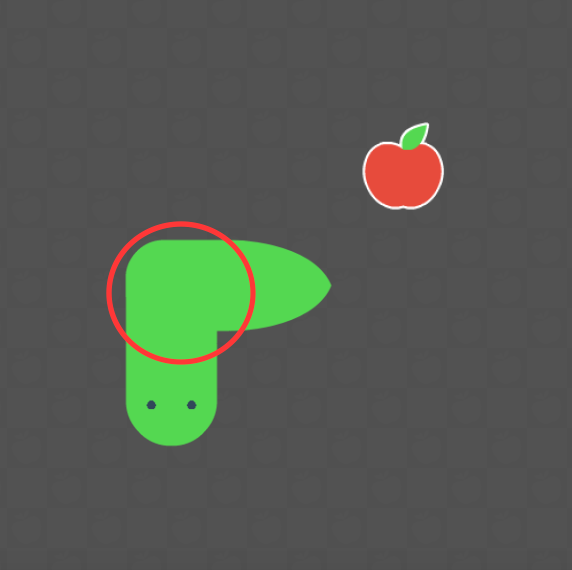
\includegraphics[width=0.15\textwidth]{Corner1.png}}
	\hspace{0.05\textwidth}
	\subfloat[Corner 2]{\label{fig:corner2}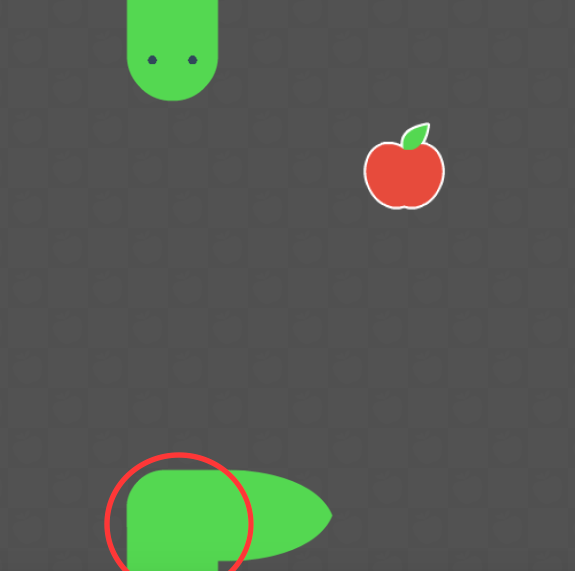
\includegraphics[width=0.15\textwidth]{Corner2.png}}
	\hspace{0.05\textwidth}
	\subfloat[Corner 3]{\label{fig:corner3}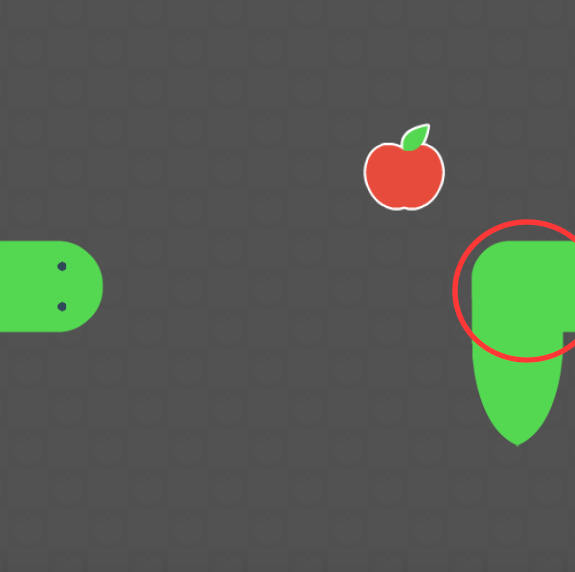
\includegraphics[width=0.15\textwidth]{Corner3.png}}
	\hspace{0.05\textwidth}
	\subfloat[Corner 4]{\label{fig:corner4}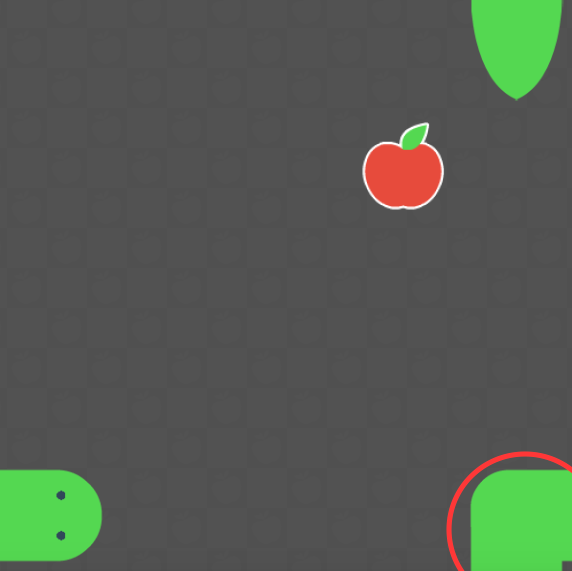
\includegraphics[width=0.15\textwidth]{Corner4.png}}
\end{figure}

\subsubsection{Lyd}

Som en mindre tilføjelse til spillet er lyd tilføjet i form af Audio-klassen. Funktionerne i Audio-klassen bruges til individuelt at spille 	

\section{Evaluering}
For at sikre stabilitet af brugergrænsefladen er spillet afprøvet i forskellige størrelser og på forskellige operativsystemer. Placeringen af komponenterne er ens i Micrsoft Windows 8.1 og dens ældre versioner, [INSERT---------]. Derimod har JButtons et lidt andet udseende på [INSEEEEERT], idet deres baggrundsfarve i dette operativsystem ikke er synlig medmindre deres kant skjules. Derudover virker de her heller ikke, hvis de tilføjes til et panel i \textit{paintComponent}-metoden. Det første problem løses ved at skjule kanten eller i stedet at bruge et ImageIcon til knappen i stedet for at give den en baggrundsfarve. Knappens funktionalitet opnås ved at tilføje knapperne i konstuktøren, men stadig med \textit{setBounds}-metoden i \textit{paintComponent}-metoden. 

Med de nye funktioner og visuelle forbedringer kørte spillet en smulle langsommere end før, mens det dog kun er synligt på svage [<-ERSTAT M SOMETHING NICER] computere. [INSERT: LØSNING HVIS VI NOGENSINDE FINDER EN : D]

-ingen brug af jbutton -> jbutton
-Se alle slangens led - gør den lidt forsinket, når den er lang
- Tjek for gentagelser



\chapter{Konklusion}
\pagebreak

\appendix
\addcontentsline{toc}{chapter}{Appendices}
\addtocontents{toc}{\protect\setcounter{tocdepth}{-1}}
\chapter{Slangens opbygning}
\section{Detaljeret oversigt af slangens opbygning}
\graphicspath{ {pics/} }
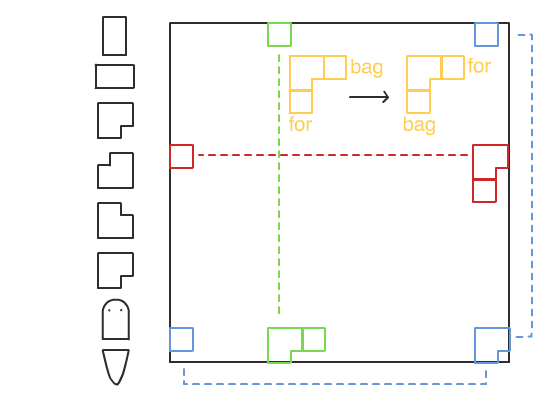
\includegraphics[width=1\textwidth]{SnakeGraphic.png}

\end{document}

